\documentclass[12pt,a4paper]{article}
\usepackage{color}
\usepackage{float}
\usepackage{graphicx}
\usepackage{indentfirst}
\usepackage{amsmath}
\usepackage{multirow}
\usepackage{url}
\usepackage{booktabs}
\def\degree{${}^{\circ}$}
\usepackage{amssymb}
\begin{document}

\vspace*{0.25cm}

\hrulefill

\thispagestyle{empty}

\begin{center}
\begin{large}
\sc{UM--SJTU Joint Institute \vspace{0.3em} \\ Introduction to Cryptography \\(VE475)}
\end{large}

\hrulefill

\vspace*{5cm}
\begin{Large}
\sc{{Project Report}}
\end{Large}

\vspace{2em}

\begin{large}
\sc{{Group 1\\
\vspace{0.5em}
bitcoin \\}}
\end{large}
\end{center}


\vfill

\begin{table}[h!]
\flushleft
\begin{tabular}{lll}
Name: Liu Niyiqiu \hspace*{2em}&
ID: 516370910118\hspace*{2em}
\\
Name: Xiang Zhiyuan \hspace*{2em}&
ID: 516370910118\hspace*{2em}
\\
Name: S \hspace*{2em}&
ID: 516370910118\hspace*{2em}
\\


\\

Date: 26 July 2019
\end{tabular}
\end{table}

\hfill

\newpage
\tableofcontents
\newpage

\section{Mining}
\subsection{Definition of Mining}
The bitcoin is a decentralized cryptocurrent. No authorities are present to authenticate each transaction. Thus the burden of verifying transactions and gathering valid transactions lies to the miners. The ultimate goal of a miner is to constitute a block by solving a mathematical problem, which will be described in the next section. To compensate the computational power spent by the miner, some bitcoins are given to the first miner that create a new block. Also, the payer in a transaction may specify a transaction fee that will be given to the miner. 
\subsection{Mathematics of Mining}
\subsubsection{Proof of Work}
The cost function is define as 
\begin{align*}
\mathcal{F}: \mathcal{S}\times \mathbb{N}^* \times \mathbb{N}^* &\longrightarrow \{\text{True, False}\}\\
(s, D, x)&\longmapsto \mathcal{F}(s, D, x)
\end{align*}
The set $\mathcal{S}$ is the set of strings. $D \in \mathbb{N}^*$ is the difficulty level of this problem and $x$ is called a nonce. $\mathcal{F}(s, D, x)$ returns true if and only if Hash($A|D|x$) starts with $D$ zeros. 


In the case of bitcoin, the hash function SHA-256 is used. In practice, $s$ and $D$ is fixed, the process of proof of work is to find a nonce $x$ such that $\mathcal{F}(s, D, x)$ returns true. An example of proof of work is shown in Fig.~\ref{fig:hash}. In this process the nonce $x$ is chosen in the order of the natural numbers.

\begin{figure}[tbph!]
	\centering
	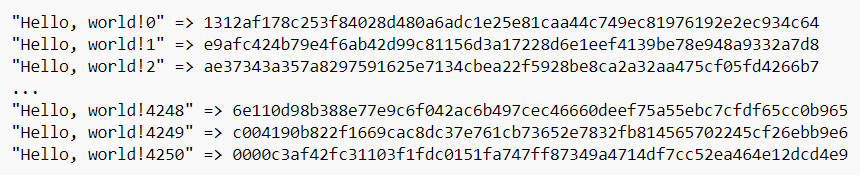
\includegraphics[width=0.9\linewidth]{Hash}
	\caption{Example of a proof of work (from bitwiki).}
	\label{fig:hash}
\end{figure}

\subsubsection{Mining a New Block}
The mining process is to solve the problem given by proof of work. At a given time, a node would gather transactions and form a block. To add this block to the block chain, the node has to solve the following problem:
\begin{align*}
&\text{Looking for a nonce $x$ such that: } Hash(s|x) < \text{target}\\
&s = s_1 | s_2 | s_3 | s_4 | s_5\\
&s_1 = \text{version}\\
&s_2 = \text{hash of previous block}\\
&s_3 = \text{hash of merkle root}\\
&s_4 = \text{timestamp }\\
&s_5 = \text{target}
\end{align*}
A block is composed of a block header and a block body. The block header is defined as $s|x$. Once a suitable nonce $x$ is found, the miner is can publish this block and add it to the block chain.
\subsection{General Procedure of Mining}
\begin{enumerate}
	\item Alice gathers the transactions and put them in a block (a block can contain approximately 4,000 transactions)
	\item Alice tries to solve the proof of work by finding a suitable nonce $x$
	\item If Alice is the first one to mine a new block, she may announce the block to the public and add it to the block chain
	\item If in the process of mining, a new block is mined by Bob. Alice abandons her block and restart step 1.
\end{enumerate}
\subsection{The Byzantine Generals' Problem}
A number of Byzantine Generals each has his own computer. They communicate through Internet to devise a plan to attack king's army. Only with a joint forces between the generals can they beat the king's army. However, several generals are spies deplored by the king. They would try to sabotage the proposed good plans. In this situation, the Byzantine General's Problem is given by how to agree upon a feasible plan to attack the king's army, given the condition that most of the generals (more than half in the case of bitcoin) are honest.


In the set up of bicoin, the Byzantine Generals' Problem is solved by the mining process at the cost of computational power (electricity). With the hard "inverse hash" step in the proof of work, the bitcoin system guarantees that no malicious user can double spend their bitcoins of forge a transaction, as will be shown in the next section.
\subsection{Double Spending and Forgery} 
Now Eve has ten bitcoins and she proposes transactions to both Bob and Alice to give them ten bitcoins each. In the meantime, there are two miners Charlie and Manuel.
\begin{enumerate}
	\item Eve announces a 10-bitcoin-transaction to  both Bob and Alice. (She only has 10 bitcoins left)
	\item Charlie first receives Eve's transaction to Alice, so he ignores Eve's transaction request to Bob.
	\item Due to delay of the Internet, Manuel first receives Eves transaction to Bob. So he ignores Eve's transaction request to Alice.
	\item Charlie and Manuel gather some transactions and both start to mine a block. 
	\item Without lose of generality, let's assume Manuel beats Charlie and solve the proof of work problem. Manuel happily add this new block to block chain. 
	\item Then Charlie would abandon his block. While gathering transactions for a new block, he would ignore Eve's transaction request because Eve's has already gave her remaining 10 bitcoins to Bob in the previous block mined by Manuel. 
\end{enumerate}

\section{Definition of Blockchain}\label{def}
Blockchain, by definition, is a growing list of records that are linked using cryptography, these records are also called as blocks. The beginning of the blockchain, which is the first block in this blockchain, is called as genesis block, every new generated block is then linked to the last block in the chain. For different blockchain, it may have different block structure, and different way to link the blocks. In cryptocurrency bitcoin, a special blockchain serves as the public ledger for all transactions on the network. 

Thus, when implementing a blockchain, the most important things are the structure of the block, and how to link the blocks.

In this part, I'll explain the block structure of the blockchain in bitcoin, and how these blocks are linked.

\subsection{Merkle Tree}

Before introducing the structure of block in bitcoin, I'll first introduce what is Merkle tree.

By definition, Merkle tree, also called as hash tree, is a tree in which every leaf node is the hash of a data block, this data block could be a file or a set of files, while for the nodes that further up in the tree, they are the hashes of their respective children. And most hash tree implementation are binary, that means their structure is a binary tree, each node can at most have two children.

For example, in Fig 1, it shows a structure of a binary hash tree. In this hash tree, it has four leaf nodes: Hash 0-0, Hash 0-1, Hash 1-0 and Hash 1-1. And we can see, for each leaf node, it contains a hash of a corresponding Data Block. For example, for Hash 0-0, it contains $hash($L1$)$, which is the hash of the Data Block L1. And for the upper nodes, like Hash 0, since Hash 0-0 and Hash 0-1 are its children, so the value contained in Hash 0 node is $hash($Hash 0-0 $||$ Hash 0-1$)$. In the same way, we can get the value contained in Hash 1 node is $hash($Hash 1-0 $||$ Hash 1-1$)$. At last, we get the root node of this hash tree, Top Hash contains $hash($ Hash 0 $||$ Hash 1$)$. Usually, we call the value of Top hash node as Merkle root hash of the Merkle tree.

Since we have learned from the course, a well performed hash function should have four properties: easy to compute, collision resistant, pre-image resistant and second pre-image resistant. And in Merkle tree, each time we calculate the hash value of a node, we are actually reinforcing the security of its children, in other words, the Merkle root hash is a hash value which contains all the information in Data Blocks. Thus, if any Data Block has been modified by even one bit, the Merkle root hash of the Merkle tree will be totally changed.

In this case, Merkle tree can be used to verify any kind of data stored, handled and transferred in and between computers, make sure the received data is undamaged and unaltered, also, is not fake.

\begin{figure}[htbp!]
	\centering
	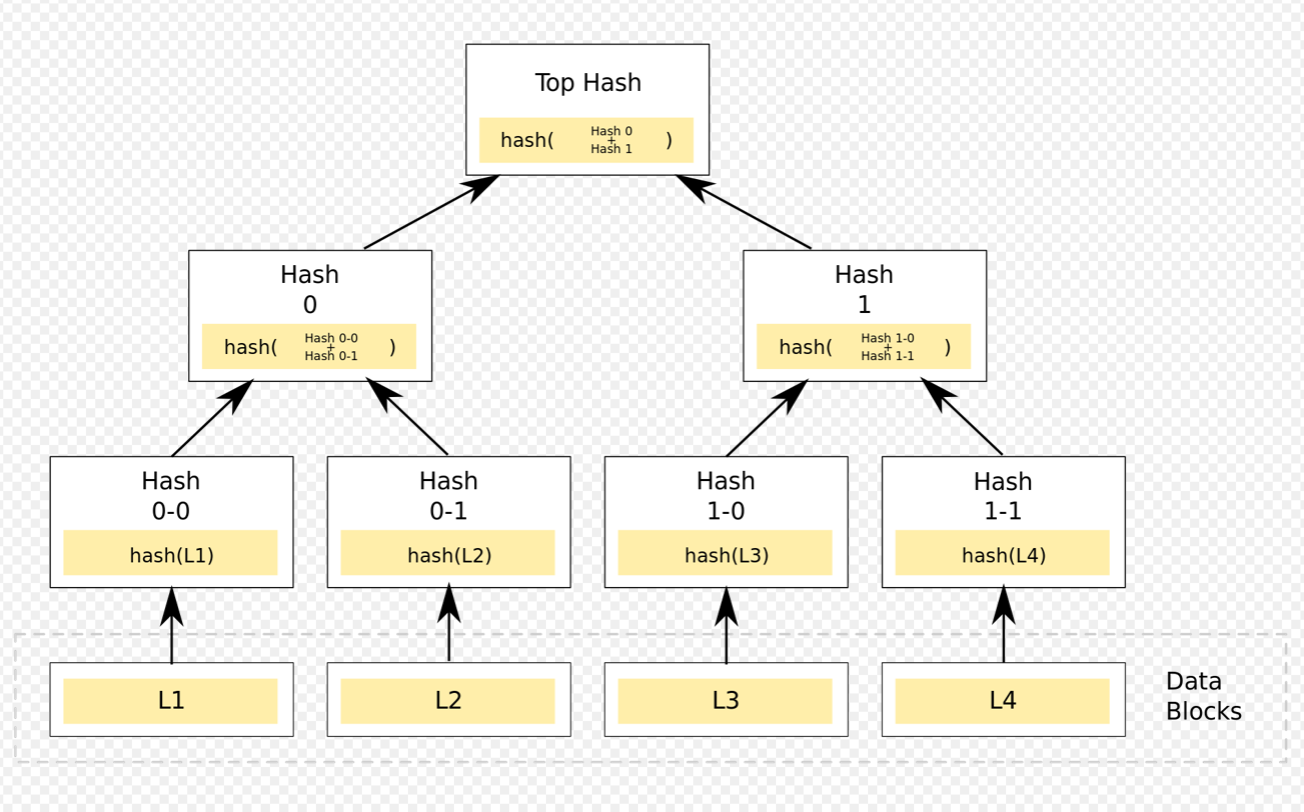
\includegraphics[width=0.7\linewidth]{hash_tree.png}
	\caption{A Binary Merkle Tree}
	\label{fig::diagram}
\end{figure}

\subsection{Block Structure}
Now that we have understood the concept of Merkle tree, and this will help us to have a better understanding of the structure of block in bitcoin system

The block in bitcoin system is made up of two parts: block header and block body.

Usually, we will define the hash of the block header as the hash of the whole block.

Block header is made up of the following parts:
\begin{enumerate}
    \item 
    version: this part record the version of the block header, which can be used to update the protocols and software.
    \item
    prevBlockHash: this part will record the cryptographic hash of previous block.
    \item
    merkleRoot: this part will record the value of Merkle root hash of the Merkle tree of all the transactions in this block.
    \item
    time: this part will record the creation timestemp of this block.
    \item
    difficultyTarget: this part will record the difficulty target of this block.
    \item
    nonce: this part will record the nonce that used to verify the proof-of-work of this block.
\end{enumerate}

And the block body is used to store the informations about transactions. On average, one block could store 500 transaction in its block body. In bitcoin system, the block body is made up of the following parts:

\begin{enumerate}
    \item 
    numTransactionsBytes: this part record the number of bytes that are used to store information about transactions.
    \item
    numTransactions: this part record the number of transactions stored in this block.
    \item
    transactions: this part will be used to store transactions.
\end{enumerate}

I will further explain why the block in bitcoin's blockchain is formed in this way, especially for the block header.

For the preBlockHash part in the block header, actually this will enable us to find the previous block by its unique hash value, and thus establish a connection between them. More details will be covered in next part, Block Linking.

And for the merkleRoot in block header, just as I have introduced before, Merkle tree can be used to verify any kind of data stored, handled and transferred in and between computers, make sure the received data is undamaged and unaltered, also, is not fake. The block will store transactions in its block body, thus, by placing all transactions into a Merkle tree and attach its Merkle root hash into the header, everyone could basing on the Merkle root hash to verify the authenticity and reliability of all the transactions in the block.

For the time part in block header, it will contain the timestamp of the creation of the block, thus it can be used to prove all transactions stored in this block should be broadcast before this timestamp.

For the difficultyTarget and nonce, these parts are related to the creation of this block, and will be covered in Mining part, so we won't explain them here.

For the block body, it contains all the transactions in the block, and all the details about the structure of transactions have been covered in Transactions part.

\subsection{Block Linking}

In this part I will explain how the blocks in bitcoin's blockchain is linked, and why we choose to link the blocks in this way.

As we have mentioned in last part, in the bitcoin system, all blocks will record the hash of previous block in its block header, and according to the definition of hash, we know that each block in a blockchain will have a unique hash, thus, the hash of the previous block is like an address, which allows us to trace back to the previous block, and by repeatedly doing this, we will eventually go back to the genesis block and cover the whole chain. This is how these block are linked to form a chain.

But why don't we just number each block, and record the corresponding number of the previous block into the block header?

The reason is that, by linking blocks in this way, we can prevent the blocks from being modified or being tampered with, thus we don't need a trusted third party to verify the security or authenticity of the block together with the transactions stored in it.

As I have mentioned, the hash of a block is the hash of its block header, and for each block, it will record the hash of previous block in its block header, that means if you modify one block, since the hash of that block also changes, you need to modify all the blocks after this, otherwise when you broadcast your falsified blockchain, other nodes in the network will fail the verification, and this falsified blockchain won't be accepted by the other nodes in the network. And in a later introduction, we will further explain why it is theoretically impossible for one to modify a block and all the other blocks after it to deceive other nodes in the network.



\section{Application of Blockchain}

Now we have already understand what is transactions in bitcoin system, and what is blockchain, how a new block is generated in bitcoin system. Thus, in this part, we will explain how the entire bitcoin system could solve some hard problems so that it can be accepted by lots of people and become one of the most widely accepted cryptocurrencys.

\subsection{Double Spending Problem}
One of the hard problem faced by many cryptocurrencys is that, how could cryptocurrency system
 prevent a node from double spending his money.
 
 For example, in bitcoin system, as we have learned, if user A want to have a transaction with user B, he wants to spend 5 bitcoins to buy something from B, he will create a new transaction basing on the previous transactions, and broadcast this transactions to the whole network, and waiting for some miners to accept this transaction and packet it into the blocks they are building. However, the problem is, if A only owns 5 bitcoins, but he also makes a transaction with C at the same time, and he wants to spend another 5 bitcoins to buy something from C, though he doesn't own enough bitcoins, but he broadcast these two transactions to the whole network nearly at the same time or within a very short time period, so how could the whole network figures out which transaction is valid, and which one is invalid? 
 
 This problem won't happen in the current monetary system. Why? Because if you are using paper money, since you cannot divide a paper into two parts and make each of them still be valuable, the double spending would never happen. Even if you are not using paper money, this problem is still impossible to happen, because there exist a trusted third party in real life, for example, the bank, or the government, every transaction you made with others will be transmit to them, and they will record every transaction of you, and if they received two transactions from you, they will basing on the received time to accept the first transaction, and for the second one, they will check you money, and find out that you don't have enough money, so the second transaction will be canceled.
 
 However, as we have mentioned, bitcoin system is decentralized, there exist no such kind of trusted third party. Thus, how could the network solve this problem?
 
 Actually, there exist a rule in bitcoin system, that is every node in the network will select the longest block chain as the correct one. Thus, when A broadcast two transactions, some nodes or miners in the network will first receive A's transaction with B, and after they verify this transaction, they will store this transaction into their own ledgers, so when they received A's transaction with C, they check and find A doesn't own enough money, so they will discard that transaction. And other nodes or miners in the network who received A's transaction with C first, they will accept this transaction and discard another one. In this case, part of the nodes or miners will accept one transaction, while the others will accept another transaction. That is when the whole system diverges.
 
 However, this situation won't last for a long time. As we have mentioned, every node in the network will select the longest block chain as the correct one and accept it. If, after a short time (according to what we have introduced in Mining part, at most after 10 mins), one of the miners in the network fortunately find out the new block, then this problem will be solve. If this lucky miner accept A's transaction with B and packet this transaction into new block, then a longer blockchain appears, so all the nodes in the network, no matter which transaction they accepted in the past, they will accept this longest blockchain and working on it, in this case, A's transaction with B is accepted by the blockchain, while the other transaction is rejected. And the same, if this lucky miner accept A's transaction with C, then the blockchain will contain A's transaction with C, and the other transaction is rejected.
 
 And you may ask, what if two lucky miners find out the new block nearly at the same time? If so, then all the other miners will record both blockchains for the time being, and each miner will select one of the two blockchains and basing on it to dig the next block. In this situation, part of the miners in the network will work on the first blockchain, while the others will work on the second blockchain, a temporary fork appears. This fork will end once a new block is found and one of the blockchains becomes longer, otherwise the fork will continue or even more forks will appear. But since the probability of two miners find a same new block is very very small, usually the fork won't last for a long time.
 
 In a conclusion, with the help of blockchain, bitcoin system could perfectly solve double spending problem.

\section{References}
\begin{enumerate}
	\item The Mathematics Behind Bitcoin, Cyril Grunspan, \url{https://webusers.imj-prg.fr/~ricardo.perez-marco/blockchain/BitcoinP7.pdf}
	\item \url{https://en.bitcoinwiki.org/wiki}
\end{enumerate}
\end{document}
